% LATEXLOG GENERATED TIMESTAMP
\documentclass{article}
\usepackage{geometry,booktabs,longtable,pdflscape,rotating,threeparttable,subcaption,graphicx,float}
\usepackage{tabularx,colortbl}
\usepackage[table]{xcolor}
\usepackage{hyperref}
\hypersetup{                           colorlinks=true,                   linkcolor={blue!50!black},                    filecolor={blue!50!black},                 urlcolor={blue!80!black},                     }                              \date{}
\geometry{verbose,letterpaper,lmargin=2.4cm,rmargin=2.4cm,tmargin=2.1cm,bmargin=2.1cm}
\newcommand{\estimand}{\widehat{\theta}}
\begin{document}
\noindent
\title{Synthetic latexlog Compatibility Report}
\maketitle
This report is generated from deterministic synthetic Stata data.
\section{Model}
The custom command produces $\estimand$ and the displayed equation is
\[\estimand=(X^{\prime}X)^{-1}X^{\prime}y,\qquad \mathrm{E}[u\mid X]=0.\]
\section{Figures}
\begin{figure}[H] 
\centering 
\caption{Synthetic Outcome and Linear Fit} 
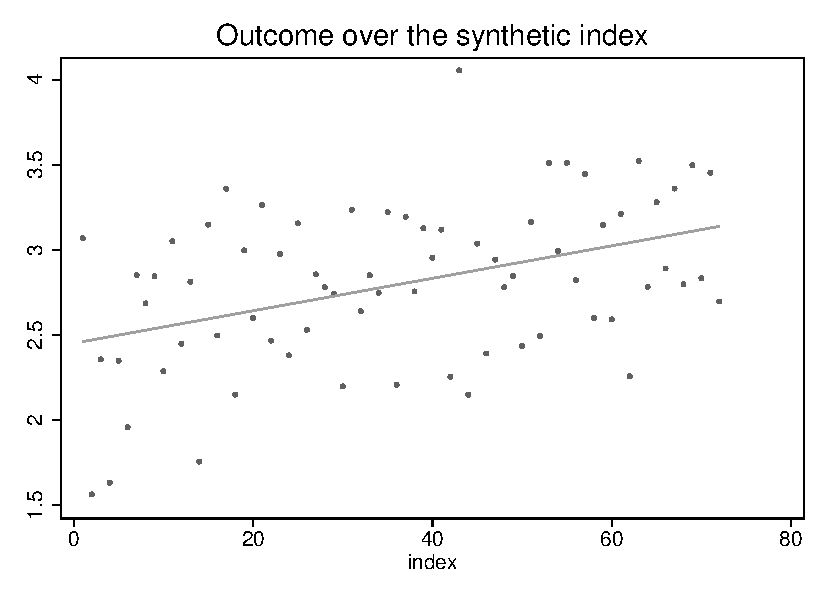
\includegraphics[width = .72\textwidth]{figures/outcome-by-index.pdf} \\ 
\begin{tabular}{p{6in}}  
\footnotesize \vspace{2pt} 
  \centering \textbf{Notes:} Deterministic synthetic observations. 
\end{tabular} 
\end{figure} 
The next PNG figure is included inline.
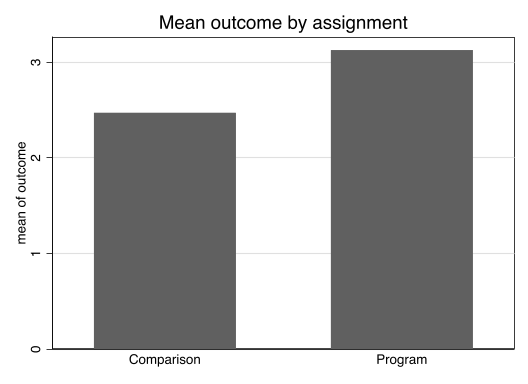
\includegraphics[width = .48\textwidth]{figures/outcome-by-treatment.png}  
\subsection{Subfigures}
\begin{figure}[H] 
\centering 
  \caption{Synthetic outcomes and exposures} 
\begin{subfigure}{.45\textwidth}
  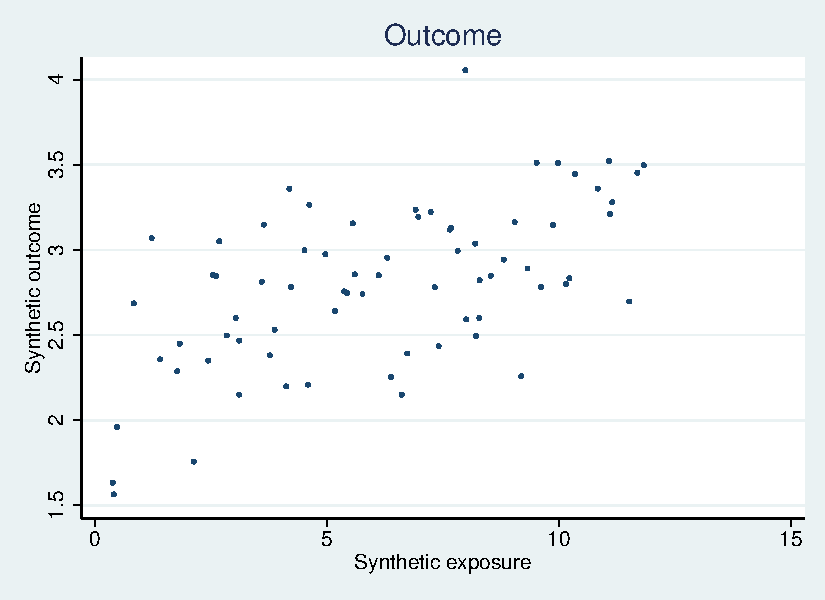
\includegraphics[width = 1.00\textwidth]{figures/panel-outcome.pdf}  
  \caption{Outcome and exposure}
\end{subfigure}
\begin{subfigure}{.45\textwidth}
  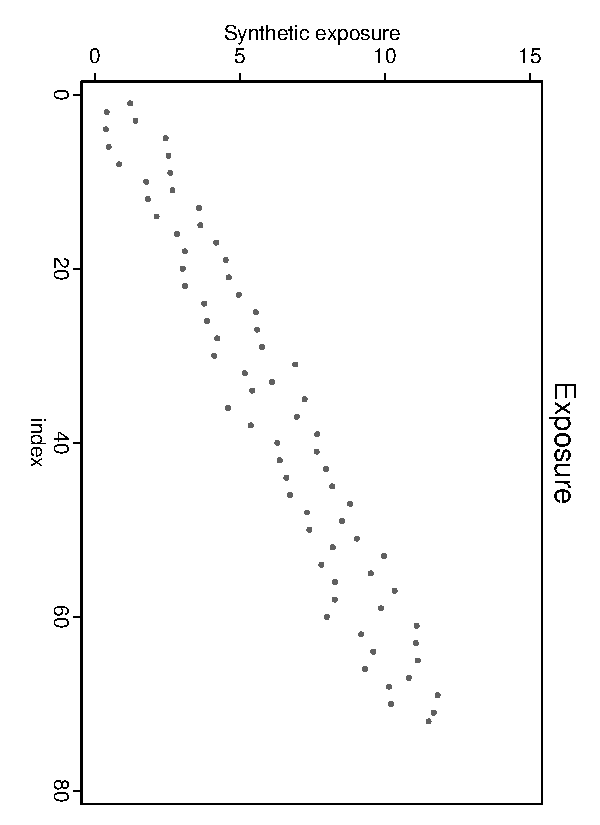
\includegraphics[width = 1.00\textwidth]{figures/panel-exposure.pdf}  
  \caption{Exposure over index}
\end{subfigure}
\begin{tabular}{p{6in}}  
 \footnotesize 
 \textbf{Notes:} All panels use the same deterministic synthetic sample. 
\end{tabular} 
\end{figure} 
\section{Tables}
\begin{table}[htbp] 
\centering 
\begin{threeparttable} 
\caption{Synthetic Outcome by Assignment and Region} 

\centering
\begin{tabular}{llll}
\toprule
\multicolumn{1}{c}{} &
  \multicolumn{3}{c}{region} \\
\multicolumn{1}{c}{} &
  \multicolumn{1}{r}{North} &
  \multicolumn{1}{r}{Central} &
  \multicolumn{1}{r}{South} \\
\midrule
\multicolumn{1}{l}{treatment} &
  \multicolumn{1}{r}{} &
  \multicolumn{1}{r}{} &
  \multicolumn{1}{r}{} \\
\multicolumn{1}{l}{\hspace{1em}Comparison} &
  \multicolumn{1}{r}{} &
  \multicolumn{1}{r}{} &
  \multicolumn{1}{r}{} \\
\multicolumn{1}{l}{\hspace{2em}Mean} &
  \multicolumn{1}{r}{2.463159} &
  \multicolumn{1}{r}{2.539315} &
  \multicolumn{1}{r}{2.416651} \\
\multicolumn{1}{l}{\hspace{2em}Standard deviation} &
  \multicolumn{1}{r}{.3268301} &
  \multicolumn{1}{r}{.348722} &
  \multicolumn{1}{r}{.4105083} \\
\multicolumn{1}{l}{\hspace{1em}Program} &
  \multicolumn{1}{r}{} &
  \multicolumn{1}{r}{} &
  \multicolumn{1}{r}{} \\
\multicolumn{1}{l}{\hspace{2em}Mean} &
  \multicolumn{1}{r}{3.093372} &
  \multicolumn{1}{r}{3.191923} &
  \multicolumn{1}{r}{3.096186} \\
\multicolumn{1}{l}{\hspace{2em}Standard deviation} &
  \multicolumn{1}{r}{.334644} &
  \multicolumn{1}{r}{.3448996} &
  \multicolumn{1}{r}{.3227683} \\
\bottomrule
\end{tabular}

 \footnotesize  
\textbf{Notes:} Means and standard deviations from synthetic data. 
\end{threeparttable} 
\end{table}
\begin{landscape}
\begin{table}[htbp] 
\centering 
\begin{threeparttable} 
\caption{Synthetic Exposure in a Landscape Tabularx Table} 

\centering
\begin{tabularx}{1.18\textwidth}{l>{\centering\arraybackslash}X>{\centering\arraybackslash}X}
\toprule
 &
  \multicolumn{2}{c}{treatment}  \\
 &
  Comparison &
  Program  \\
\midrule
region &
   &
    \\
\hspace{1em}North &
  5.691014 &
  6.8481  \\
\hspace{1em}Central &
  5.596109 &
  6.609192  \\
\hspace{1em}South &
  5.209268 &
  7.204909  \\
\bottomrule
\end{tabularx}

 \footnotesize  
\textbf{Notes:} Selected columns use the tabularx X column type. 
\end{threeparttable} 
\end{table}
\end{landscape}
\section{Conclusion}
Figures, tables, notes, custom commands, and mathematics resolved successfully.

\end{document}
